\chapter{From ten to four dimensions: scales and supersymmetry}
\label{ch:L1}
\lecturedate{Lecture of 5 November 2026}

This first lecture of the second part of the course is an overview. Its purpose is to give a global picture of how one goes from ten-dimensional superstring theory to the four-dimensional world we observe, before the following lectures fill in the details. Two questions organise it. The first is quantitative: when six of the ten dimensions are compact, which energy scales appear, and in which window of energies can we trust which effective description? The answer is a hierarchy of three scales, the Planck mass, the string scale and the Kaluza--Klein scale, controlled by two numbers, the string coupling $g_s$ and the volume $\Vol$ of the extra dimensions in string units. The second question is qualitative: how much of the supersymmetry of ten-dimensional string theory survives in four dimensions? The answer depends on the holonomy of the compact space, and it is what singles out Calabi--Yau manifolds.

\section{Where we stand and where we are going}
\label{sec:L1-aims}

The first part of the course, Prof.\ Ling Lin's module, described the string from the point of view of its worldsheet. The fundamental object is a vibrating string, and quantising it means quantising the two-dimensional field theory that lives on the surface it sweeps out, the worldsheet, whose fields are the spacetime coordinates $X^M$ of the string. This is a two-dimensional conformal field theory. It has a Weyl symmetry, and the requirement that this symmetry has no anomaly fixes the dimension of spacetime, $D = 26$ for the bosonic string. The spectrum of the bosonic string contains a tachyon, a sign that the theory is unstable. To get rid of it one adds fermions on the worldsheet. The result is the superstring, whose critical dimension is $D=10$. The Gliozzi--Scherk--Olive (GSO) projection removes the tachyon, and the theory turns out to be supersymmetric not only on the worldsheet but also in spacetime. The quantum states of the string form a tower of modes, a few of them massless and the others massive, and each of them corresponds to a spacetime field; among the massless modes of the closed string are the metric $G_{MN}$, the Kalb--Ramond two-form $B_{MN}$ and the dilaton $\phi$.

Besides closed strings there are open strings, whose endpoints are attached to extended objects, the D$p$-branes, of any dimension up to that of spacetime. The open strings ending on a brane describe fields that live on it, in particular gauge fields, and on a stack of $N$ coincident branes they give a non-abelian gauge theory with gauge group $U(N)$.
There are five consistent perturbative superstring theories, which differ in how the spectrum is chosen: type I, types IIA and IIB, in which worldsheet fermions are added for both the left- and the right-moving degrees of freedom of the closed string, and the two heterotic theories, with gauge groups $SO(32)$ and $E_8\times E_8$, in which only the right-movers are supersymmetrised. Perturbatively they look different, but they are related by dualities, some of which exchange a strongly coupled theory with a weakly coupled one, and they are understood as different limits of a single underlying theory, M-theory (\cref{sec:L2-dualities}). Loop amplitudes are sums over Riemann surfaces of increasing genus, which replace the Feynman diagrams of field theory; since the string has a finite size, which acts as a natural cutoff, they have no ultraviolet divergences.

From here one could follow many directions: the quantum properties of each of the five theories, their mathematical structure, black holes in ten or fewer dimensions. This part of the course follows one of them, \emph{string compactifications}: how to reproduce our four-dimensional world, with the Standard Model and cosmology, starting from ten-dimensional string theory. The idea is to take spacetime to be four-dimensional Minkowski space times a compact six-dimensional space, and to go to energies below the inverse size of the extra dimensions, where they can no longer be seen. What remains is a four-dimensional effective theory with local supersymmetry, a supergravity theory of the kind met in the supersymmetry course, with the important difference that it is not written down by hand: it is derived from a consistent theory of quantum gravity. Its physics depends strongly on the geometry and the topology of the extra dimensions, so we shall need some differential geometry and Calabi--Yau manifolds, and D-branes will play an essential role in reproducing the non-abelian gauge theories seen in nature. The module covers the low-energy effective action of string theory, D-brane actions and dualities, type II compactifications on Calabi--Yau manifolds, flux compactifications and moduli stabilisation, supersymmetry breaking in string models, and the basic principles of string cosmology.

We shall see that the way down from ten to four dimensions is not unique. There is a \emph{landscape}, or a multiverse, of solutions, each corresponding to a different four-dimensional universe. The goal is to find at least one that reproduces what we know, the Standard Model and cosmology, and possibly also offers solutions to the open problems recalled at the beginning of the supersymmetry course: inflation, dark matter, dark energy, the hierarchy problem and supersymmetry breaking.

The subject is vast, and this part of the course is necessarily dense. Rather than deriving everything systematically from a set of assumptions, which would cover one topic in depth but give a very partial view of the subject, the aim is a global understanding of the whole picture, with details to be studied afterwards where one is interested. The first lectures are therefore largely qualitative, meant to build intuition for how things go; later lectures return to the main steps with explicit computations, together with the mathematical background they need (differential forms, complex manifolds, branes and the dualities that generalise electric--magnetic duality).

\paragraph{References.} The following books, reviews and lecture notes cover the material of this part of the course, and much more:
\begin{enumerate}
  \item L.~E. Ibáñez and A.~M. Uranga, \emph{String Theory and Particle Physics: An Introduction to String Phenomenology}~\cite{IbanezUranga};
  \item A.~Hebecker, \emph{Naturalness, String Landscape and Multiverse}, lecture notes freely available online~\cite{Hebecker};
  \item R.~Blumenhagen, B.~Körs, D.~Lüst and S.~Stieberger, \emph{Four-dimensional string compactifications with D-branes, orientifolds and fluxes}, a long review~\cite{BKLS};
  \item lecture notes by J.~Louis, available on his website~\cite{Louis};
  \item D.~Baumann and L.~McAllister, \emph{Inflation and String Theory}, a book whose lecture-note version is available online~\cite{BaumannMcAllister};
  \item M.~Cicoli, J.~P. Conlon, A.~Maharana, S.~Parameswaran, F.~Quevedo and I.~Zavala, \emph{String cosmology: from the early universe to today}~\cite{StringCosmoReview}.
\end{enumerate}
The first four are oriented towards particle physics and the low-energy limit of string theory. The last two are oriented towards cosmology, which is a particularly promising arena for testing string theory, because some cosmological questions, inflation above all, can only be addressed reliably in an ultraviolet-complete theory. The review~\cite{StringCosmoReview} starts with an introduction to compactifications and then follows the whole cosmological history, from inflation through reheating to dark matter and dark energy.

The exam consists of a twelve-minute slide presentation on a topic chosen by the student, from either part of the course, followed by questions on that topic. Reproducing a topic as it was presented in the lectures can earn up to 29/30; for 30 or 30 cum laude something more is expected, for which references can be asked to the lecturers. A mark can be turned down once.

\section{Superstring theory as a theory of quantum gravity}
\label{sec:L1-qg}

Superstring theory is a consistent quantum theory, and the reason for the interest in it is that it is a consistent theory of quantum \emph{gravity}. Its massless spectrum contains a symmetric tensor field $G_{MN}(X)$, the metric: there is a massless spin-two particle, the graviton, and so there is gravity, in a theory whose loop amplitudes are finite. But string theory is not only a theory of gravity. It also contains gauge interactions and matter, basically all the rest of physics, so that it is a candidate for a unified description of all interactions, and it is a framework large enough that other approaches to quantum gravity may turn out to be contained in it.

The theory is consistent because two potential problems are absent. There are no tachyons, thanks to the GSO projection, and there are no states of negative norm. The second requirement is the absence of a Weyl anomaly on the worldsheet, and it fixes the number of spacetime dimensions to the critical dimension
\begin{equation}
  D = 10 .
  \label{eq:L1-D10}
\end{equation}
String theory is the only theory we know that predicts the number of spacetime dimensions. The prediction is, at first sight, wrong, since we see four dimensions. But it is not so bad: the answer is a positive integer, and it could have been worse.

\begin{addition}
\emph{Where $D=10$ comes from.} In the covariant quantisation of the superstring the worldsheet theory contains, besides the $D$ bosons $X^M$ and their $D$ fermionic partners, the ghosts that come from fixing the worldsheet diffeomorphisms and local supersymmetry. Each field contributes to the central charge of the Virasoro algebra: $1$ for each boson, $\tfrac12$ for each Majorana fermion, $-26$ for the $bc$ ghosts and $+11$ for the $\beta\gamma$ superghosts. The Weyl anomaly is proportional to the total, $c_{\text{tot}} = \tfrac32 D - 15$, and vanishes only for $D=10$, i.e.\ for a ``matter'' theory of central charge $c = 15$. The same condition makes the BRST charge nilpotent, $Q_B^2 = 0$, which is what guarantees that the negative-norm states introduced by covariant quantisation decouple from the physical spectrum. For the bosonic string the same counting gives $D - 26 = 0$.
\end{addition}

\section{Compactification and the Kaluza--Klein scale}
\label{sec:L1-KK}

To make contact with the real world we must study \emph{string compactifications}. Ten-dimensional Minkowski space $\R^{1,9}$ is a solution of string theory, but there are others, in which ten-dimensional spacetime is the product of four-dimensional Minkowski space and a six-dimensional manifold,
\begin{equation}
  X_{10} = \R^{1,3}\times Y_6 ,
  \label{eq:L1-X10}
\end{equation}
where $Y_6$ is a \emph{compact} space: a six-sphere, a six-dimensional torus, or something more complicated. Its volume $\mathrm{Vol}(Y_6)$ has dimensions of a length to the sixth power, so its $-1/6$ power is an energy, the \emph{Kaluza--Klein scale},
\begin{equation}
  \MKK \coloneqq \frac{1}{\mathrm{Vol}(Y_6)^{1/6}} .
  \label{eq:L1-MKK-def}
\end{equation}
$\MKK$ is the energy above which one starts to see the extra dimensions; equivalently, $1/\MKK$ is the length scale below which they become visible. We expect
\begin{equation*}
  \MKK \gg E_{\mathrm{LHC}} \sim 1\TeV ,
\end{equation*}
the energies probed at the LHC, and this explains why we have not seen extra dimensions.

The idea is easiest to picture in two dimensions. Take a spacetime that is a cylinder, with one extended direction and one direction curled up into a circle, and look at it from very far away: one sees a line, not the circle (\cref{fig:L1-cylinder}). In the same way, it is not so strange to expect that at every point of our four-dimensional spacetime there is a six-dimensional curled-up space that we do not see, simply because it is too small.

\begin{figure}[tbp]
  \centering
  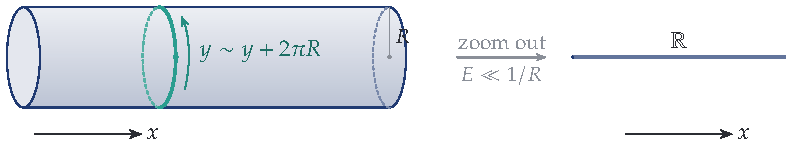
\includegraphics{fig_L1-cylinder}
  \caption{A cylinder $\R\times S^1$ seen from close by and from far away: at distances much larger than its circumference, or energies much lower than $1/R$, it looks like a line. Every point of the line carries a small circle, as every point of $\R^{1,3}$ carries a copy of $Y_6$.}\label{fig:L1-cylinder}
\end{figure}

\begin{addition}
\emph{The Kaluza--Klein tower.} The name of $\MKK$ comes from the tower of four-dimensional particles that a single higher-dimensional field gives, as met in the supersymmetry course. For a massless scalar $\Phi(x,y)$ on $\R^{1,3}\times S^1$, with $y\sim y+2\pi R$, the Fourier expansion $\Phi = \sum_{n\in\Z}\varphi_n(x)\,e^{iny/R}$ turns the five-dimensional wave equation into four-dimensional Klein--Gordon equations for the modes $\varphi_n$ with masses $m_n = |n|/R$. At energies $E\ll1/R$ only the zero mode $\varphi_0$ can be produced, and the theory looks four-dimensional. On a six-dimensional torus with six circles of radius $R$, $\mathrm{Vol}(Y_6) = (2\pi R)^6$ and the lightest massive modes have $m = 1/R = 2\pi/\mathrm{Vol}(Y_6)^{1/6}$. Thus \cref{eq:L1-MKK-def} fixes $\MKK$ only up to a factor of order one (here $2\pi$), and for a less symmetric $Y_6$ the precise spectrum depends on its shape, not only on its volume; what matters for us is the scaling with the volume.
\end{addition}

\section{The string scale and the Planck scale}
\label{sec:L1-scales}

Let us now place the relevant scales on an energy axis. Somewhere high up is the four-dimensional Planck mass $\Mp$; somewhere below it is the \emph{string scale}, the inverse of the string length,
\begin{equation}
  \Ms = \frac{1}{\ls} ,\qquad \ls = 2\pi\sqrt{\alpha'} .
  \label{eq:L1-Ms-def}
\end{equation}
The string length is set by the only free parameter of string theory, $\alpha'$, which determines the string tension, $T = 1/(2\pi\alpha')$. When the string is quantised, its vibrational modes give states that are either massless or have masses set by $1/\sqrt{\alpha'} = 2\pi\Ms$, growing with the level of excitation. Why have we drawn $\Ms$ below $\Mp$? To answer this, we have to relate the two.

\subsection{The ten-dimensional action and the dilaton}

From the scattering amplitudes of strings, at tree level and at loop level, one can reconstruct the effective action of the massless modes of the string in ten dimensions. Among its terms is the ten-dimensional Einstein--Hilbert term
\begin{equation}
  S_{10} \supset \frac{1}{2\kappa_{10}^2}\int\dd^{10}X\,\sqrt{-G}\;e^{-2\phi}\,R_{10} ,
  \qquad
  \frac{1}{2\kappa_{10}^2} = \frac{2\pi}{\ls^8} = 2\pi\,\Ms^8 ,
  \label{eq:L1-S10}
\end{equation}
where $R_{10}$ is the Ricci scalar built out of the ten-dimensional metric $G_{MN}$, and $\phi$ is the \emph{dilaton}, another massless mode of the string. The factor $e^{-2\phi}$ multiplying the Ricci scalar means that this is the action in the \emph{string frame} (see the conventions).

The remarkable property of the dilaton is that its vacuum expectation value fixes the strength of the interactions among strings, the \emph{string coupling},
\begin{equation}
  g_s = e^{\langle\phi\rangle} .
  \label{eq:L1-gs}
\end{equation}
The string coupling is therefore not a parameter that one can choose by hand, as one chooses $\alpha'$. It is a function of the expectation value of a field: when the dilaton moves, the strength of the string interactions changes.

The action in \cref{eq:L1-S10} is the tree-level contribution. As usual, it receives perturbative loop corrections, and on top of those non-perturbative ones, and their size relative to the tree-level action is controlled by $g_s$. If the string coupling is large the loop corrections are large, and the tree-level action cannot be trusted. If instead $\langle\phi\rangle$ is large and negative, the string coupling is small, and in the limit $\langle\phi\rangle\to-\infty$ all loop corrections become negligible. If one did not want to assume anything, one would have to compute all possible quantum corrections, beyond tree level, perturbative and non-perturbative, and then see what dynamics the complete theory gives: this would really be a dream, and it is not doable in practice. What one does instead is to \emph{assume} that the string coupling is small, so that to a first approximation the tree-level part is enough, and then check a posteriori that the potential for $\phi$ has a minimum where $g_s$ is indeed small. Since the value of $\phi$ is determined dynamically, this is a consistency condition, not a choice; if it fails, loops should have been included from the very beginning. We shall see that there is a way to make sure that the condition holds, which is nice. In summary, to trust perturbation theory we need
\begin{equation}
  g_s \ll 1 \qquad\Longleftrightarrow\qquad \langle\phi\rangle \to -\infty .
  \label{eq:L1-weak}
\end{equation}

\begin{addition}
\emph{Why $e^{-2\phi}$, and the Einstein frame.} In string perturbation theory a closed-string amplitude on a worldsheet of genus $g$ (a sphere with $g$ handles) is weighted by $g_s^{2g-2} = g_s^{-\chi}$, where $\chi = 2-2g$ is the Euler characteristic. The tree-level action comes from the sphere, $\chi=2$, which is the origin of the factor $e^{-2\phi}$ in \cref{eq:L1-S10}; the one-loop terms (the torus, $\chi=0$) come without dilaton factor, and so on. The kinetic term of $G_{MN}$ is mixed with that of the dilaton through this factor. A Weyl rescaling $G_{MN} = e^{(\phi-\phi_0)/2}G^E_{MN}$, with $\phi_0 = \langle\phi\rangle$, removes it: in ten dimensions $\sqrt{-G}\,R_{10}[G] = e^{2(\phi-\phi_0)}\sqrt{-G_E}\,R_{10}[G_E] + (\text{derivatives of }\phi)$, so that the factor $e^{-2\phi}$ becomes the constant $e^{-2\phi_0} = g_s^{-2}$ and the action takes the Einstein--Hilbert form in the Einstein-frame metric $G^E_{MN}$. With this choice the two frames coincide in the vacuum. For completeness, the full bosonic action of the NS--NS fields in the string frame is
\begin{equation*}
  S_{\mathrm{NS}} = \frac{1}{2\kappa_{10}^2}\int\dd^{10}X\,\sqrt{-G}\;e^{-2\phi}\Bigl(R_{10} + 4\,\partial_M\phi\,\partial^M\phi - \frac{1}{2\cdot3!}H_{MNP}H^{MNP}\Bigr),
\end{equation*}
with $H = \dd B$ the field strength of the Kalb--Ramond field; the R--R fields and the fermions add further terms, which we shall meet in the following lectures.
\end{addition}

\subsection{Dimensional reduction and the Planck mass}

We now perform the \emph{dimensional reduction} of \cref{eq:L1-S10} on the background of \cref{eq:L1-X10}, going to energies below the Kaluza--Klein scale. The ten-dimensional metric factorises into a four-dimensional piece and a six-dimensional one,
\begin{equation}
  G_{MN}\,\dd X^M\dd X^N = g_{\mu\nu}(x)\,\dd x^\mu\dd x^\nu + g_{mn}(y)\,\dd y^m\dd y^n ,
  \label{eq:L1-ansatz}
\end{equation}
so that $\sqrt{-G} = \sqrt{-g_4}\,\sqrt{g_6}$ and $R_{10} = R_4 + R_6$. Keeping the term with the four-dimensional Ricci scalar, the action becomes
\begin{equation}
  S_{10} \supset 2\pi\Ms^8\underbrace{\int_{Y_6}\dd^6y\,\sqrt{g_6}}_{\mathrm{Vol}(Y_6)}\;\int\dd^4x\,\sqrt{-g_4}\;e^{-2\phi}\,R_4 .
  \label{eq:L1-reduction}
\end{equation}
There are other contributions, in particular the one with the internal Ricci scalar $R_6$, which we ignore for now (see the addition below).
In the vacuum the dilaton takes its expectation value and can be taken outside the integral:
\begin{equation}
  S_{10} \supset \underbrace{2\pi\Ms^8\,\mathrm{Vol}(Y_6)\,e^{-2\langle\phi\rangle}}_{=\,\Mp^2/2}\int\dd^4x\,\sqrt{-g_4}\,R_4 .
  \label{eq:L1-vacuum}
\end{equation}
This is the usual four-dimensional Einstein--Hilbert action, and its coefficient is the Planck mass, $\Mp^2/2$. Writing the volume in terms of a dimensionless quantity $\Vol$, the volume in string units, $\mathrm{Vol}(Y_6) = \Vol\,\ls^6$, and using $e^{-2\langle\phi\rangle} = g_s^{-2}$ and $\ls^6 = \Ms^{-6}$, we find
\begin{equation}
  \boxed{\;\Mp^2 = 4\pi\,\frac{\Vol}{g_s^2}\,\Ms^2\;}
  \qquad\Longrightarrow\qquad
  \Ms = \frac{g_s}{\sqrt{4\pi\Vol}}\,\Mp \simeq g_s\,\frac{\Mp}{\sqrt{\Vol}} .
  \label{eq:L1-MP-Ms}
\end{equation}

Since $\ls$ is the only parameter of string theory, \cref{eq:L1-MP-Ms} allows us to trade it for the Planck mass. Conceptually $\Ms$ is the fundamental scale and $\Mp$ a derived one, but $\Mp$ is the one we know, so in practice we fix $\Mp\simeq2.4\times10^{18}\GeV$ and derive everything else from it. The other two quantities in \cref{eq:L1-MP-Ms} are not parameters at all: $g_s$ is the expectation value of the dilaton, and we shall see that $\Vol$ is the expectation value of another field, the volume modulus. In the end everything is derived dynamically.

\begin{addition}
\emph{What was dropped, and the Einstein frame in four dimensions.} Three simplifications are hidden in \cref{eq:L1-reduction}. First, the product form of the metric, \cref{eq:L1-ansatz}, ignores the possibility that the size of $\R^{1,3}$ depends on the point of $Y_6$ (a warp factor), which will become important in flux compactifications. Second, the term $\int_{Y_6}\dd^6y\sqrt{g_6}\,R_6$, which we dropped, contributes to the four-dimensional scalar potential; it vanishes when $Y_6$ is Ricci-flat, as Calabi--Yau manifolds are (\cref{sec:L1-holonomy}). Third, we have set the dilaton and the volume to constants. If they are allowed to vary along $\R^{1,3}$, as the fields they are, the coefficient of $R_4$ in \cref{eq:L1-reduction} is $2\pi\Ms^2\,\Vol(x)\,e^{-2\phi(x)}$, which is not constant, and the four-dimensional action is not in the Einstein frame. A Weyl rescaling of the four-dimensional metric by $e^{-2\phi}\Vol$, relative to its vacuum value, brings it to that frame; it is the origin of the powers of $\Vol$ in the four-dimensional scalar potential that we shall meet later.

\emph{The ten-dimensional Planck mass.} In the ten-dimensional Einstein frame the coefficient of the Einstein--Hilbert term defines a ten-dimensional Planck mass, $\frac{1}{2\kappa_{10}^2g_s^2} \equiv \frac12M_{10}^8$, i.e.
\begin{equation}
  M_{10}^8 = \frac{4\pi}{g_s^2}\,\Ms^8 ,\qquad
  M_{10} = (4\pi)^{1/8}\,g_s^{-1/4}\,\Ms ,\qquad
  \Mp^2 = M_{10}^8\,\mathrm{Vol}(Y_6) .
  \label{eq:L1-M10}
\end{equation}
The last relation is the general statement that the four-dimensional strength of gravity is diluted by the volume of the extra dimensions. Above $\MKK$ gravity is ten-dimensional, and it is $M_{10}$, not $\Mp$, that sets the scale at which it becomes strong. For $g_s<1$ and $\Vol>1$ it lies between the two: $\Ms < M_{10} < \Mp$.
\end{addition}

\section{Perturbative control: string loops and \texorpdfstring{$\alpha'$}{alpha'} corrections}
\label{sec:L1-control}

\Cref{eq:L1-MP-Ms} tells us that
\begin{equation}
  \Ms \ll \Mp \simeq 2.4\times10^{18}\GeV
  \qquad\text{for}\qquad g_s \ll 1 \quad\text{and}\quad \Vol \gg 1 .
  \label{eq:L1-hierarchy-conditions}
\end{equation}
(The board rounds $\Mp$ to $10^{18}\GeV$.) The first condition is that of \cref{eq:L1-weak}, needed to trust the string loop expansion. The second condition, that the volume be large in string units, is needed to trust another kind of perturbation theory. To see why, write the inverse volume as
\begin{equation}
  \frac{1}{\Vol} = \frac{\ls^6}{\mathrm{Vol}(Y_6)} = \frac{(2\pi)^6\,\alpha'^3}{\mathrm{Vol}(Y_6)} .
  \label{eq:L1-invV}
\end{equation}
The limit of large volume is the limit in which $\alpha'$ is small compared with the size of the extra dimensions, $\alpha'^3\ll\mathrm{Vol}(Y_6)$.
A string of fixed size moving in a volume that is huge compared with it is the same as a volume of fixed size in which the string length is sent to zero. But $\ls\to0$ is the limit in which strings become point-like particles, and in which the standard Feynman diagrams of quantum field theory are recovered from the string diagrams. Corrections in $1/\Vol$ are therefore genuinely \emph{stringy} corrections: they tell us that the fundamental objects are strings, not point-like particles.

So the effective theory receives two kinds of corrections, controlled by two different expansion parameters. The first are \emph{string loops}, the sums over Riemann surfaces of higher genus, with expansion parameter $g_s$; in the point-particle limit they reduce to the loop diagrams of quantum field theory. The second, with expansion parameter $1/\Vol$, do not look like loop corrections from the point of view of the spacetime quantum field theory. They are tree-level corrections, but with higher derivatives, like the operators of dimension five, six, seven and higher that one generates at tree level in field theory by integrating out heavy particles; here the heavy modes that are integrated out are the massive string modes. They are called \emph{$\alpha'$ corrections}, and controlling them requires $1/\Vol\ll1$. From the point of view of spacetime they are higher-derivative corrections; from the point of view of the worldsheet theory they are \emph{worldsheet loops}, the loops of the two-dimensional field theory, which are counted by $\alpha'$. In the regime $g_s\ll1$, $\Vol\gg1$ one can trust the effective theory and neglect both string loops and higher-derivative corrections, at least to a first approximation.

\begin{addition}
\emph{The size of the $\alpha'$ corrections.} Each power of $\alpha'$ in the ten-dimensional effective action comes with two more derivatives. On $Y_6$, of typical length $L = \mathrm{Vol}(Y_6)^{1/6}$, two derivatives cost $1/L^2$, so each order is suppressed by $\alpha'/L^2 = 1/\bigl((2\pi)^2\Vol^{1/3}\bigr)$. In type II string theory supersymmetry forbids the corrections at orders $\alpha'$ and $\alpha'^2$, and the first correction to the gravitational action is a term of the form $\alpha'^3R^4$, quartic in the curvature. Relative to the tree-level term it is of order $\alpha'^3/L^6 = 1/\bigl((2\pi)^6\Vol\bigr)$, which is precisely the quantity of \cref{eq:L1-invV}. Its effect on the four-dimensional theory, computed by Becker, Becker, Haack and Louis~\cite{BBHL}, will be an essential ingredient of the Large Volume Scenario. Strictly speaking, control of the $\alpha'$ expansion requires all the curvature radii of $Y_6$ and the sizes of all of its cycles, not only its total volume, to be large in string units.
\end{addition}

\section{A hierarchy of scales and of effective theories}
\label{sec:L1-hierarchy}

We can now complete the picture of the energy scales, shown in \cref{fig:L1-scales}. At the top is $\Mp\simeq 2.4\times10^{18}\GeV$, and the string scale is below it, at a value we do not know, since it depends on $g_s$ and $\Vol$ through \cref{eq:L1-MP-Ms}. At energies above $\Ms$ we see the whole ten-dimensional string theory: all the string resonances can be produced. The theory we shall study is type IIB string theory, which at present looks the most promising for obtaining phenomenology from string theory, for reasons that start to be explained in \cref{ch:L2}.

At energies below the string scale one remains in ten dimensions, but one can no longer produce the massive string modes, only the massless ones. What is left is no longer a string theory but a quantum field theory of point particles in ten dimensions, the fields that correspond to the massless modes of the string, with spectrum and interactions fixed by string theory. Since we started from a superstring this theory is supersymmetric, and since it contains gravity its supersymmetry is local: it is a ten-dimensional supergravity. For the type IIB string it is \emph{type IIB supergravity}, with ten-dimensional $\mathcal N=2$: there are two supersymmetry generators, two Majorana--Weyl spinors of the same chirality. ``Type IIB'' means that the field content is the massless spectrum of the type IIB string, not something chosen by hand.

Going to still lower energies we reach the Kaluza--Klein scale, below which the extra dimensions are invisible and the theory is four-dimensional. By \cref{eq:L1-MKK-def,eq:L1-MP-Ms},
\begin{equation}
  \MKK = \frac{1}{\mathrm{Vol}(Y_6)^{1/6}} = \frac{\Ms}{\Vol^{1/6}} \simeq g_s\,\frac{\Mp}{\Vol^{2/3}} ,
  \label{eq:L1-MKK}
\end{equation}
where the power of the volume is $\tfrac16+\tfrac12 = \tfrac23$, and, keeping the factor of \cref{eq:L1-MP-Ms}, $\MKK = g_s\Mp/(\sqrt{4\pi}\,\Vol^{2/3})$. The Kaluza--Klein scale is below the string scale, $\MKK<\Ms$: written in terms of $\Mp$, the two scales are $g_s\Mp/\Vol^{2/3}$ and $g_s\Mp/\Vol^{1/2}$, and for large volume $\Vol^{2/3}>\Vol^{1/2}$; equivalently, $\MKK/\Ms = \Vol^{-1/6}<1$. In the regime of \cref{eq:L1-hierarchy-conditions}, in which we trust the effective theory, the hierarchy of scales is therefore
\begin{equation}
  \MKK < \Ms < \Mp ,\qquad
  \frac{\MKK}{\Ms} = \frac{1}{\Vol^{1/6}} ,\qquad
  \frac{\Ms}{\Mp} = \frac{g_s}{\sqrt{4\pi\Vol}} .
  \label{eq:L1-hierarchy}
\end{equation}
Below $\MKK$ one obtains a four-dimensional supergravity theory, described, as in global supersymmetry, by a Kähler potential and a superpotential.

As a reminder of the conventions: since our Einstein frame coincides with the string frame in the vacuum, $\Vol$ in \cref{eq:L1-MP-Ms,eq:L1-MKK} is the Einstein-frame volume as well. In references that define the Einstein frame without subtracting $\phi_0$ the same relations appear as $\Ms = g_s^{1/4}\Mp/\sqrt{4\pi\Vol'}$ and $\MKK\simeq\Mp/\Vol'^{2/3}$, in terms of a volume $\Vol' = g_s^{-3/2}\Vol$ (see the conventions).

\begin{figure}[tbp]
  \centering
  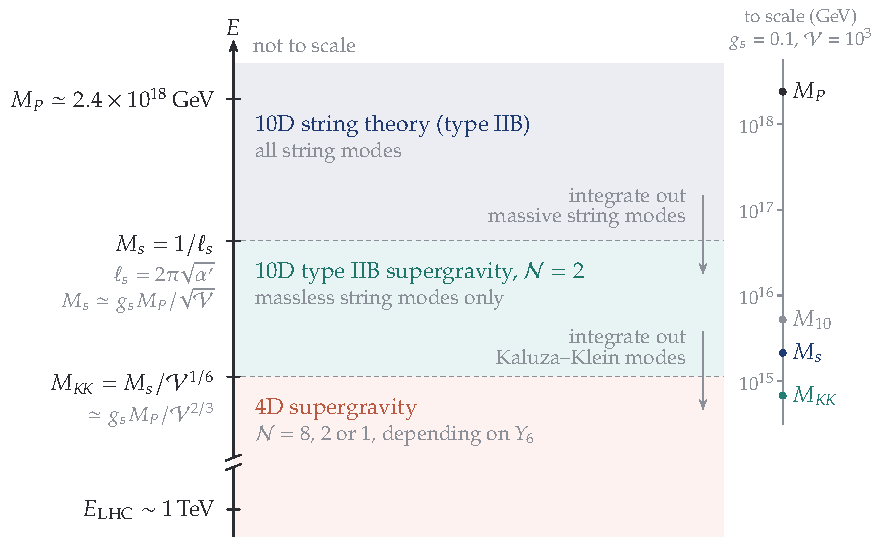
\includegraphics{fig_L1-scales}
  \caption{The hierarchy of scales of a string compactification and the effective description valid in each window of energies. The ratios are fixed by $g_s$ and $\Vol$ through \cref{eq:L1-hierarchy}.}\label{fig:L1-scales}
\end{figure}

\section{How much supersymmetry survives: holonomy}
\label{sec:L1-holonomy}

The number of supersymmetries in four dimensions depends, of course, on the number of supersymmetries in ten dimensions, but it also depends on the topology of $Y_6$. The supersymmetry generators are spinors: in type IIB supergravity two ten-dimensional Majorana--Weyl spinors. Given one such spinor in ten dimensions, one can ask how many four-dimensional spinors it corresponds to, and the answer depends on the compact space. This is what singles out the famous Calabi--Yau manifolds. The statements in this section are made in words; we shall prove them later in this part of the course.

Consider first the simplest situation, a flat internal manifold, the six-dimensional torus $T^6$. In this case the largest amount of supersymmetry is preserved: one Majorana--Weyl spinor in ten dimensions corresponds to four spinors in four dimensions, and the two of type IIB give four-dimensional $\mathcal N=8$ supergravity,
\begin{equation}
  Y_6 = T^6 ,\quad \Hol(T^6) = \{\one\}
  \qquad\Longrightarrow\qquad \text{4D } \mathcal N=8 .
  \label{eq:L1-T6}
\end{equation}
The property of $T^6$ that matters here is that it is a space of trivial \emph{holonomy}: its holonomy group contains only the identity.

The holonomy is a simple notion. Take a manifold, choose a closed path in it starting and ending at a point $p$, take a vector at $p$ and parallel-transport it around the path, as in \cref{fig:L1-holonomy}. When it gets back to $p$ the vector has the same length, but it need not be the same vector. On a flat manifold it always comes back to itself, but on a curved manifold it is in general rotated. A different closed path gives in general a different rotation. The \emph{holonomy group} is the set of all the transformations that relate the original vector to the transported one, for all possible closed paths. If the holonomy group contains only the identity, the vector always comes back to itself, as in the flat case; this is the trivial situation of the torus, which is flat.

\begin{figure}[tbp]
  \centering
  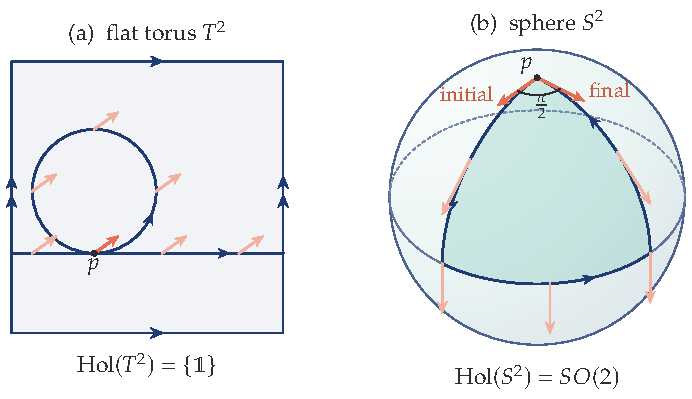
\includegraphics{fig_L1-holonomy}
  \caption{Parallel transport around closed loops. On a flat torus a vector always returns to itself, so the holonomy is trivial. On a sphere a vector carried around a closed loop returns rotated, here by $\pi/2$; the holonomy group collects all such rotations.}\label{fig:L1-holonomy}
\end{figure}

Now notice the beauty of this result. In the supersymmetry course we saw that $\mathcal N=8$ is the largest amount of supersymmetry a four-dimensional theory can have: beyond it, the supermultiplets contain massless particles of spin higher than two, which have no consistent interactions and are not seen in nature. String theory never gives more than $\mathcal N=8$, so a consistent theory reproduces this result automatically. Compactification of type IIB string theory on $\R^{1,3}\times T^6$ is a perfectly good solution of the theory. But it does not describe our world, because $\mathcal N=8$ is too much supersymmetry. The world needs at most $\mathcal N=1$ at high energies: in four-dimensional theories with $\mathcal N\ge2$ the fermions cannot be chiral, while those of the Standard Model are (see also \cref{sec:L1-questions}). The supersymmetry must be reduced, and the way to reduce it is what selects Calabi--Yau manifolds.

If instead of $T^6$ the space $Y_6$ is a \emph{Calabi--Yau manifold}, whose holonomy group is $SU(3)$, then one Majorana--Weyl spinor in ten dimensions gives a single spinor in four dimensions, and type IIB gives four-dimensional $\mathcal N=2$ supergravity:
\begin{equation}
  Y_6 = \text{Calabi--Yau} ,\quad \Hol(Y_6) = SU(3)
  \qquad\Longrightarrow\qquad \text{4D } \mathcal N=2 .
  \label{eq:L1-CY}
\end{equation}
This is why Calabi--Yau manifolds, the six-dimensional manifolds of $SU(3)$ holonomy, became famous: they break the largest possible amount of supersymmetry while preserving some of it, which is what is needed to make contact with the real world.

\begin{addition}
\emph{Why the holonomy decides.} On $\R^{1,3}\times Y_6$ the ten-dimensional Lorentz group is broken to $SO(1,3)\times SO(6)$, and the Majorana--Weyl representation $\mathbf{16}$ of $SO(1,9)$ decomposes as
\begin{equation}
  \mathbf{16} = (\mathbf 2,\mathbf 4)\oplus(\bar{\mathbf 2},\bar{\mathbf 4}) ,
  \label{eq:L1-spinor-decomp}
\end{equation}
where $\mathbf 2$ and $\bar{\mathbf 2}$ are the two Weyl spinors of $SO(1,3)$, and $\mathbf 4$ and $\bar{\mathbf 4}$ the two chiral spinors of $SO(6)$, the fundamental and antifundamental of $SU(4)\simeq\mathrm{Spin}(6)$. The Majorana condition relates the two terms, so a ten-dimensional supersymmetry parameter has the form $\epsilon(x,y) = \zeta(x)\otimes\eta(y) + \text{c.c.}$, with $\zeta$ a four-dimensional Weyl spinor and $\eta$ a spinor on $Y_6$. A supersymmetry is preserved by the background if the variations of the fermions vanish in it. With no fluxes and a constant dilaton the only condition comes from the gravitino, $\delta\psi_M = \nabla_M\epsilon = 0$, which requires $\eta$ to be covariantly constant on $Y_6$, $\nabla_m\eta = 0$. A covariantly constant spinor is unchanged by parallel transport around any loop, so it is a singlet of $\Hol(Y_6)$ acting on the $\mathbf 4$. Each such singlet $\eta$ gives one four-dimensional supersymmetry for each ten-dimensional Majorana--Weyl generator. For $T^6$ all four components are singlets, and type IIB gives $2\times4 = 8$ supersymmetries. For $\Hol = SU(3)\subset SU(4)$, $\mathbf 4\to\mathbf 3\oplus\mathbf 1$ has a single singlet, and type II gives $\mathcal N=2$; the heterotic and type I strings, which have a single Majorana--Weyl supersymmetry in ten dimensions, give $\mathcal N=1$ directly, which is how Calabi--Yau manifolds first entered string theory~\cite{CHSW} (\cref{sec:L2-heterotic}). An intermediate case is $\Hol = SU(2)$, e.g.\ $Y_6 = K3\times T^2$, with $\mathbf 4\to\mathbf 2\oplus\mathbf 1\oplus\mathbf 1$ and $\mathcal N=4$ from type II. Finally, a compact Kähler manifold of complex dimension three has $\Hol\subseteq U(3)$, and $\Hol\subseteq SU(3)$ is equivalent to Ricci-flatness; by Yau's theorem a Ricci-flat Kähler metric exists, in each Kähler class, precisely when the first Chern class vanishes. This is the usual definition of a Calabi--Yau manifold, and Ricci-flatness guarantees that the $R_6$ term dropped in \cref{eq:L1-reduction} vanishes.
\end{addition}

To reach four-dimensional $\mathcal N=1$ one more step is needed. Half of the degrees of freedom have to be projected away: one has to cut the spectrum. The operation that does it in type IIB is the \emph{orientifold projection}. It reverses the orientation of the strings and identifies different modes of the string with each other, and keeping only the combinations invariant under it projects out half of the spectrum, and with it half of the supersymmetries. Type IIB string theory on a Calabi--Yau orientifold gives four-dimensional $\mathcal N=1$ supergravity. We shall understand later in more detail what this operation means.

\begin{addition}
\emph{The orientifold projection.} Type IIB string theory is invariant under worldsheet parity $\Omega_p$, which reverses the orientation of the string and exchanges its left- and right-moving modes. Gauging this symmetry, i.e.\ keeping only the states invariant under it, gives type I string theory. In an orientifold, $\Omega_p$ is combined with an involution $\sigma$ of the compact space, $\sigma^2 = 1$, and the theory is restricted to the states invariant under the combination; the name joins ``orientation'' and ``orbifold''. For a Calabi--Yau manifold $\sigma$ is taken holomorphic and isometric, and two choices preserve four-dimensional $\mathcal N=1$~\cite{GrimmLouis}:
\begin{equation*}
  \mathcal O = (-1)^{F_L}\,\Omega_p\,\sigma^* \quad\text{with}\quad \sigma^*\Omega = -\Omega ,
  \qquad\qquad
  \mathcal O = \Omega_p\,\sigma^* \quad\text{with}\quad \sigma^*\Omega = +\Omega ,
\end{equation*}
where $\Omega$ is the holomorphic three-form of the Calabi--Yau and $(-1)^{F_L}$ the spacetime fermion number of the left-movers. The fixed loci of $\sigma$ are \emph{orientifold planes}: in the first case O3-planes, at points of $Y_6$, and O7-planes, wrapping four-cycles; in the second case O5- and O9-planes. Unlike D-branes, O-planes are not dynamical, and they carry negative tension and negative Ramond--Ramond charge. This will make them essential for the consistency (tadpole cancellation) of flux compactifications, and the O3/O7 case is the setting of the moduli-stabilisation scenarios studied later in the course.
\end{addition}

All these statements hold at the compactification scale. This scale, as we have seen, is not known, but it is expected to be very high, perhaps $10^{18}$, $10^{16}$ or $10^{15}\GeV$. At that scale, depending on the manifold on which the theory is compactified, one has four-dimensional $\mathcal N=8$, $\mathcal N=2$ for a Calabi--Yau, or $\mathcal N=1$ for a Calabi--Yau orientifold. The remaining task is then to break the last $\mathcal N=1$ to $\mathcal N=0$, at low energy, around the TeV scale, and dynamically.

The plan of this part of the course is to explain these steps: start from ten-dimensional type IIB supergravity and see how to go down to four-dimensional theories with $\mathcal N=8$, $\mathcal N=2$ and finally $\mathcal N=1$, discussing along the way the geometric notions, such as holonomy, that they require.

\section{Questions and discussion}
\label{sec:L1-questions}

The lecture ended with questions from the students. We reproduce them here with the answers, because they touch on themes that will return throughout the course.

\question{Do we have any reason to think that $g_s$ is small?}

There is no a priori reason for the string coupling to be small. The region $g_s\ll1$ is the one in which we can perform computations, but nature does not need to be in the region where we can compute. There are, however, indications that it is small, and they come from observation: everything we see in nature so far looks weakly coupled. There are many small numbers in what we know. The electromagnetic coupling $\alpha_{\mathrm{em}} = e^2/4\pi$ is about $1/137$ at the energies of our experiments; the Yukawa couplings are small, that of the electron being $y_e\simeq3\times10^{-6}$; in cosmology, the density fluctuations of the cosmic microwave background are of order $10^{-5}$. We shall see that gauge and Yukawa couplings are functions of the string coupling (and of the other moduli), so their smallness is an indication that $g_s$ is small.

But the dilaton is a field, and a field can have different configurations, different vacua. Some vacua may correspond to universes in which $g_s$ is large. They would still be solutions of string theory, just not our universe, and in fact in most of the solutions we know $g_s$ is not small. Once there are different solutions one must also understand, cosmologically, why one of them is realised in nature rather than another, or whether several are, in which case we are in a kind of multiverse and must ask how our universe is connected to the other parts. These are deep questions.

Small $g_s$ is also required from the point of view of the theory, to trust the computations, so the phenomenological and the theoretical requirements point in the same direction. In principle one would start from ten-dimensional string theory and compute all quantum effects: a tree-level part, loop corrections and non-perturbative corrections. Dimensionally reducing the full result would then give the complete four-dimensional $\mathcal N=1$ theory, with all quantum effects included. This is unfeasible. If the string coupling is small, however, one can keep only the leading-order result, knowing that the corrections one cannot compute are negligible. As said above, this is an assumption that has to be checked: the dilaton turns out to be a scalar field in four dimensions, one has to compute its potential and find where it has a minimum, since cosmologically the field is expected to end up there, and that minimum must lie at weak coupling. In most solutions this is not the case, but we shall see that in a subset of solutions it is guaranteed. We focus on those, both for the consistency of the theory and because they are good candidates to reproduce the Standard Model.

\question{If we had started from type IIA, which is not chiral in ten dimensions, could we still obtain a chiral theory in four dimensions?}

Yes: one can also start from type IIA and obtain chiral four-dimensional theories. Chirality depends on the dimension: when we say that the world is chiral we mean that it is chiral in four dimensions, and a theory that is chiral in ten dimensions need not be chiral in four. Type IIB, for instance, is chiral in ten dimensions, but compactified on $T^6$ it gives four-dimensional $\mathcal N=8$ supergravity, which is not chiral. A four-dimensional theory can be chiral only when it has $\mathcal N=1$ (or no supersymmetry). Type IIA is not chiral in ten dimensions, but when it is compactified down to four-dimensional $\mathcal N=1$ it can give a chiral theory as well. The reason why people mostly focus on type IIB rather than type IIA is that the latter is technically more complicated, not that it is excluded; we shall come back to this.

\question{The real requirement of the worldsheet theory is not ten dimensions but a central charge $c=15$. Are there options we are not considering, some conformal field theory that is not geometrical?}

Yes. The worldsheet conformal field theory describing the ``matter'' must have $c=15$, and ten free bosons with their fermionic partners are only one way of achieving it. One should think of string theory, or M-theory, as a big space of theories in which one can move, finding different configurations. At some points the configuration can be described geometrically, as $\R^{1,9}$ or as $\R^{1,3}\times Y_6$; at other points there is no geometric description. An example is the limit in which the volume of the extra dimensions goes to zero, where one finds conformal field theory limits with no geometric interpretation.

\question{Is there a reason to believe that our universe is not in one of these limits?}

Yes. In those limits there is no hierarchy. All scales are of order the string scale, and all couplings are of order one. To reproduce our universe one needs hierarchies: the string scale below the Planck scale, supersymmetry broken at a much lower scale, couplings that are small.

\begin{addition}
The counting behind $c=15$ is the one of the addition after \cref{eq:L1-D10}: the ghosts contribute $-26+11=-15$, so the rest of the worldsheet theory must contribute $+15$, with $\mathcal N=1$ worldsheet supersymmetry. In a compactification $\R^{1,3}\times Y_6$ the four flat directions contribute $\tfrac32\times4=6$, and the internal theory must have $c=9$. For a Calabi--Yau this is a supersymmetric sigma model on $Y_6$, but any conformal field theory with $c=9$ (and, for spacetime supersymmetry, $\mathcal N=2$ worldsheet supersymmetry) will do. A famous example is the Gepner model, built from $\mathcal N=2$ minimal models, which describes the quintic Calabi--Yau at a point of small volume where the geometric description has broken down.
\end{addition}

A remark of the lecturer's own belongs here. Everything said so far is put in by hand. We have assumed the background $\R^{1,3}\times Y_6$ and allowed deformations of $Y_6$: it can be a torus or a Calabi--Yau manifold, and we shall allow the Calabi--Yau to change in size, for example to have a different volume, or in shape. A change of shape at fixed size is like deforming a doughnut into a teacup: there is still one hole, one handle, and the volume may stay the same, but the shape changes. These deformations will be the moduli of the compactification (\cref{sec:L2-moduli}). It would be very nice to understand dynamically why we end up in this background rather than in something else, for example $\R^{1,4}\times Y_5$, but this is very hard, and we are not able to do it yet: it requires the whole non-perturbative M-theory, not perturbative string theory.

\question{Why do we need to understand M-theory to determine $Y_6$?}

Think of the difference between first and second quantisation in quantum field theory. The first-quantised description is the worldline formalism, in which one follows one particle at a time; to describe as many particles as one likes one needs a quantum field theory. In the first part of the course the string was introduced as a generalisation of the worldline, the worldsheet, and this formulation of string theory is a kind of first-quantised version. What one would like is a string field theory, with a field whose excitations are strings, and a complete formulation of this kind, able to describe the theory non-perturbatively, is not available.

\question{Would matrix theories, such as the BFSS model, count as string field theories?}

Matrix theories, such as the BFSS matrix model of Banks, Fischler, Shenker and Susskind, in which M-theory is described by the quantum mechanics of a large number of D0-branes, are proposals for the heart of M-theory, and branes play a crucial role in them; there are many papers on these proposals, but no consensus on the right formulation. The point is that what we can actually do is perturbative, and a simple way to see the problem is a quantum-mechanical system with two vacua. Everything we have done here studies one vacuum. Perturbation theory around it allows us to deform it, for instance to deform the Calabi--Yau, but never to reach the other vacuum, which could be, say, $\R^{1,4}\times Y_5$. What interpolates between two vacua in quantum mechanics is an instanton, a tunnelling effect, which is non-perturbative because it is not a small perturbation around either vacuum, and to describe it one needs the whole picture. Perturbative string theory around one vacuum gives, at low energy, one quantum field theory, for instance four-dimensional $\mathcal N=1$ supergravity from type IIB; around another vacuum, another quantum field theory. Connecting the two, and understanding cosmologically how the different vacua were populated in the first place, would require a description that interpolates between the different solutions of string theory.

\question{In such a description, should one see a smooth transition from, say, type IIB to the $E_8\times E_8$ heterotic string?}

Yes, one should. But the situation is even more complicated than this. Even without leaving type IIB, string theory gives many, many solutions, the landscape. They were found within type IIB because this is the limit in which computations can be done and things are under control. Sticking to this setting, one finds many different quantum field theories, all based on Calabi--Yau manifolds (more precisely, orientifolds) in type IIB, differing by the fluxes that we shall meet later; and relating them to each other, even within type IIB, would require understanding all possible connections between vacua.

The present approach is more humble. Out of all the solutions, let us at least find one that looks like our universe: one with non-abelian gauge theories like the Standard Model, the right cosmology, and so on. There are many that look like our universe. The second question is what happens to the other solutions. This question can be asked regardless of string theory, and in quantum field theory the situation is even worse: one can write down infinitely many quantum field theories, changing the gauge group or the spectrum of fields, all perfectly viable as quantum field theories, but disconnected from one another; the choice is just ours. In string theory we do not yet know how many consistent solutions there are, but at the moment their number seems to be finite, and in principle one can understand, quantum mechanically and at the non-perturbative level, how they are connected. We are far from that. A more immediate programme, in the most promising setting for phenomenology, is to study all the possible solutions and understand their common features, and then to see whether they lead to predictions: if all of them contain a new particle that we should see in nature, for example, or if none of them does, one can confront this with data.
